\chapter{Proposal}
\label{ch:prop}

This thesis proposes a new FSS embedded method termed \WKII. Its overall goal is to identify relevant feature subsets and as much as possible information about dependencies that explain significant patterns hidden in the data. This method treats the features estimation and patter discovery as an optimization problem. It uses a \EDA~ to explore the search space and the goodness of each candidate is assessed by a learning technique.  Each candidate represents, for the \Learner, a relevance estimation for its feature space. The better the candidate portrays the relevant features in the feature space the better the classification accuracy and fitness score obtained. \\
The main components of \WKII~ are depicted in Figure \ref{fig:im02}. The \emph{data} is the sample of observed variables for a given problem;  The \emph{Bivariate Bernoulli Distribution} is the probability distribution estimated by the \EDA~ algorithm whose parameters are the marginal probabilities $P(\bar{x} = 1 )$ and the contingency tables of the pair-wise dependencies from the variables.

\begin{figure}[ht]
	\centering
		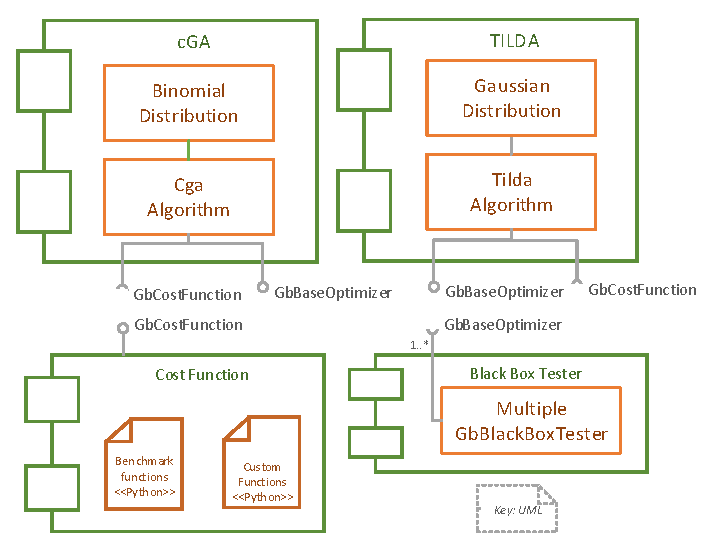
\includegraphics{components}
	\caption{The components involved in \WKII .}
	\label{fig:im02}
\end{figure}

The \EDA~ is a technique to infer the parameters and structure of the bivariate probability distribution by estimating its parameters iteratively from a pool of promising candidate weight vectors; the distribution and candidates are adjusted within a framework of a stochastic population-based evolutionary algorithm. The \WK~ \emph{Cost Function} acts as an mediator between the \EDA~ and the \Learner. It takes each candidate \(\bar{w}\) from the \EDA~ as a relevance estimator of the \Learner's feature space. If the \Learner~ is a \emph{Weighted Kernel Classifier} the weight vector \(\bar{w}\) becomes the weights for the \emph{Weighted Kernel}. Therefore the fitness of each candidate \(\bar{w}\) is the classification accuracy measurement from the cross-validation.\\

A general flowchart of \WKII~ is shown in Figure \ref{fig:im03}.  There, the \emph{Bivariate EDA} generates the candidates to explore the search space.  Each candidate is assessed by the \Learner~ and top ranked are selected by the \EDA to reestimate the bivariate distribution.  This flow is repeated until the probability distribution converge or a finalization criterion is met.  As a result the \EDA provides the best solution found with a weigh vector \(\bar{w}\) representing the variables relevances and the dependencies as a hierarchical forest. The pseudo-code is summarized in Algorithm \ref{alg:idea}.

\begin{figure}[ht]
	\centering
		\includegraphics[scale=0.7]{flowchart}
	\caption{\WKII~ flowchart.}
	\label{fig:im03}
\end{figure}

\begin{algorithm}[ht]
	\caption{\textsf{Pseudocode of the method described in this proposal}}
	\begin{algorithmic}
		\REQUIRE Given a dataset $\cD$, a weighted kernel $\kappa_\omega$ and a learner $\cA$
		\STATE Let $\beta$ represents a bivariate bernoulli probability distribution initialized with an independent joint distribution. Let $\cB$ represents the best solution.
		\REPEAT 
			\STATE $\bar{\Omega} \gets$ Sample $k$ candidates from $\beta$ 
			\FOR{$\bomega_j \in \Omega$}
				\STATE Cross Validation: $cv_j \gets \cA (\cD, \kappa_{\omega_j})$
				\STATE Classification Accuracy: $ca_j \gets$ C\cA$(cv_j)$
			\ENDFOR
			\STATE $\bar{\Omega}' \gets$ get\_top\_ranked$(\bar{\Omega},\bar{ca})$
			\STATE Update best solution if needed:  $\cB \gets update(\cB,\bar{\Omega}')$
			\STATE Re-estimate distribution: $\beta \gets$ re\_estimate$(\bar{\Omega}')$
	\UNTIL $\beta$ has converged or maximum number of evaluations reached
	\RETURN Distribution $\beta$ and best solution found $\cB$ 
	\end{algorithmic}
	\label{alg:idea}
\end{algorithm}

\section{Why \TILDA~and \GB~?}

During the exploration and development phases of \WKII~ two important contributions were achieved: \TILDA~ and \GB. On one hand, \TILDA~ was the result of the analysis performed on \EDA s algorithm.  We identify \cGA~ as a memory efficient algorithm with promising results on problems of millions of variables.  However, it was only conceived to work on a discrete domain $[0,1]$.  Therefore  we mixed the \cGA 's memory-efficient capabilities and the well-known \PBILc~ continuous domain \EDA~ in a new algorithm named \emph{Tiny Incremental Learning Density Estimation Algorithm} (\TILDA) and its arithmetic-coding version \TILDAC (a detailed explanation can be found in chapter \ref{ch:tilda}). On the other hand, after an exploration of machine learning frameworks and tools in order to build upon them \WKII, we found \Orange: An open-source component-based software framework, featuring visual and scripting interfaces for many machine learning algorithms. By design \Orange~ provides clear extensibility points named \emph{widgets and add-ons}, to integrate as plug-ins new developed algorithms.  \Orange did not provided tools for optimization nor for \EDA s, one of the main components needed for \WKII . Therefore we introduced \GB, an \Orange~add-on with visual components for stochastic search-based optimization, feature selection and machine learning. Its main purpose was to provide an user-friendly workbench for building and testing  \WKII upon its versatile visual front-end of and the powerful reuse and glue principles of component-based software development. Architecture of the toolbox and implementation details are given in chapter \ref{ch:goldenberry}, including description and working examples for all its components. 